\section{Results}
We can now look into the results of our work and show how we can create our different variations of the game. As we have already discussed, we can give the player three different abilities and likewise we can give the boss two different abilities, but we can also choose not to have a boss. The room can take a combination of four weathers, and based on those, we can meet different weather effects in the game variations. We can thus create \textbf{36} different variations.

\begin{figure}[H]
	\centering
	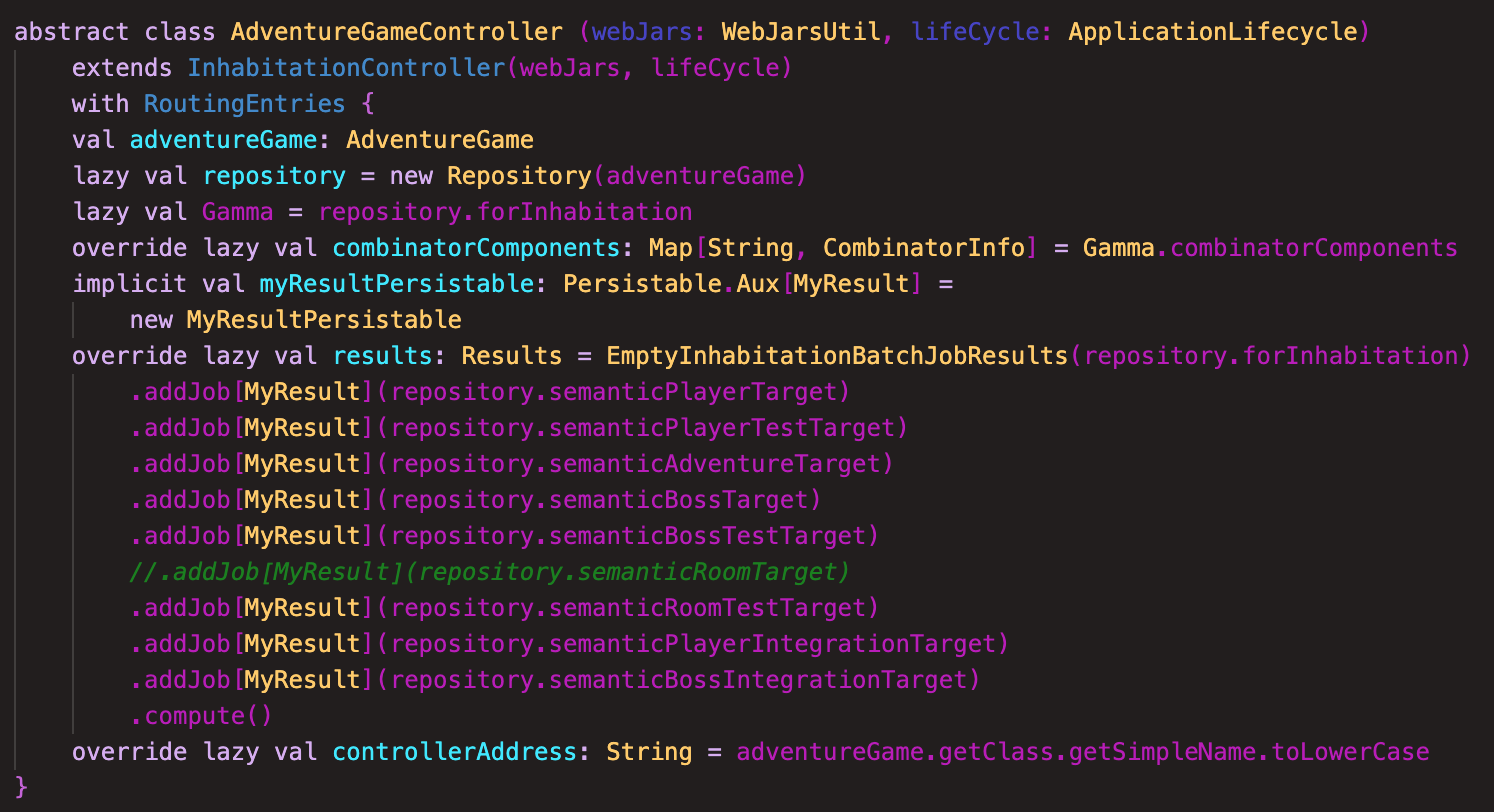
\includegraphics[width=\linewidth]{Materials/Results/AdventureController}
	\caption{In the \textit{AdventureGameController} we can see what jobs we are scheduling and thus what we want synthesized.}
	\label{Controller}
\end{figure}
In \autoref{Controller} we see \textit{AdventureGameController} in which we add the jobs we want done. Each job correspond to a synthesis we want done, and so if we are only interested in creating a player we could remove the other jobs.

\begin{figure}[H]
	\centering
	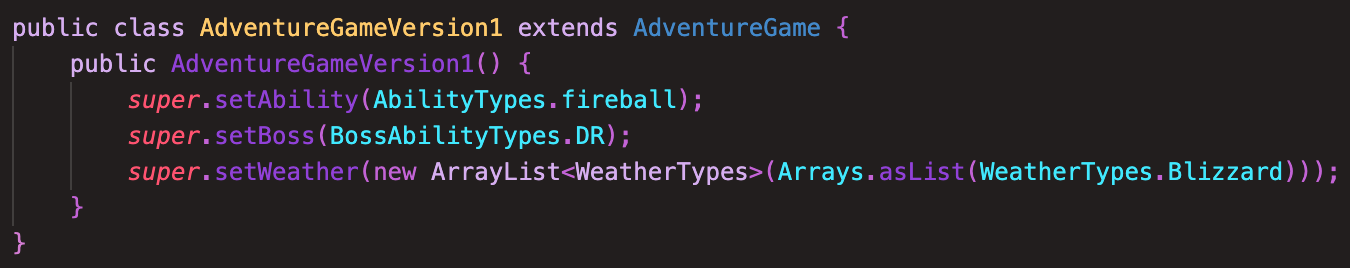
\includegraphics[width=\linewidth]{Materials/Results/AdventureVariation}
	\caption{By setting the \textit{AdventureGame} fields we can create different variation of our game. Here is shown a variation where the player has the fireball, the boss has the damage reduction ability and the possible weather effects would be blizzard.}
	\label{version1}
\end{figure}

To alter the variation we synthesize we need to look at a concrete class which extends our \textit{AdventureGame} class. We can here look at \textit{AdventureGameVersion1} which is seen in \autoref{version1}. We here see the player having the fireball ability, the boss having the damage reduction ability, and the possible weather effects being blizzard.

\begin{wrapfigure}{R}{0.6\linewidth}
	\centering
	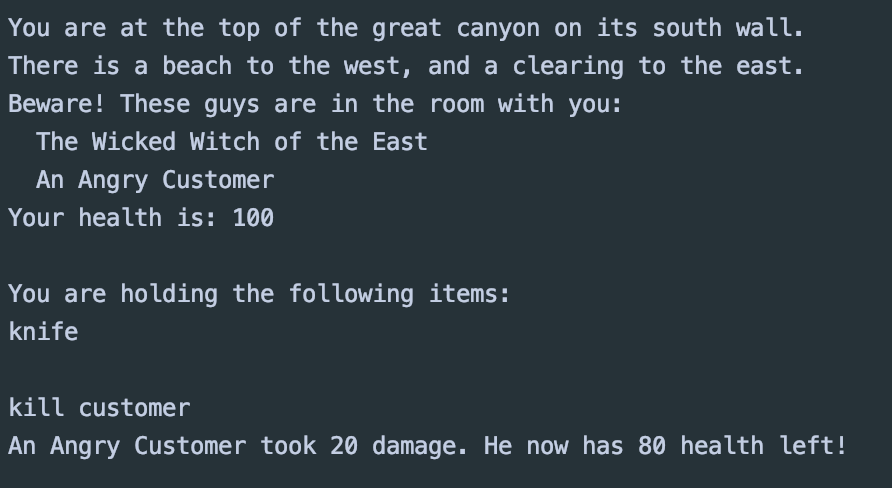
\includegraphics[width=\linewidth]{Materials/Results/AttackingCustomer}
	\caption{We see that the player with the knife can attack the Angry Customer.}
	\label{sc1}
\end{wrapfigure}
In the following we will showcase that the initial application can be synthesized and played. Here we are focusing on \autoref{sc1}, \autoref{sc2} and \autoref{sc3}. As we start the game we see that we can not hit other players in the room with us. This is because we need the knife to attack with, as we do not have the fireball in the initial application. With the knife we can now begin stabbing both other players, but also the evil customer monster. The concept for hitting the 'Wicked Witch' is the same, but here we need the water. As this is all there is to the game in the initial application, our showcase of the initial application is done.

\begin{figure}[H]
	\centering
	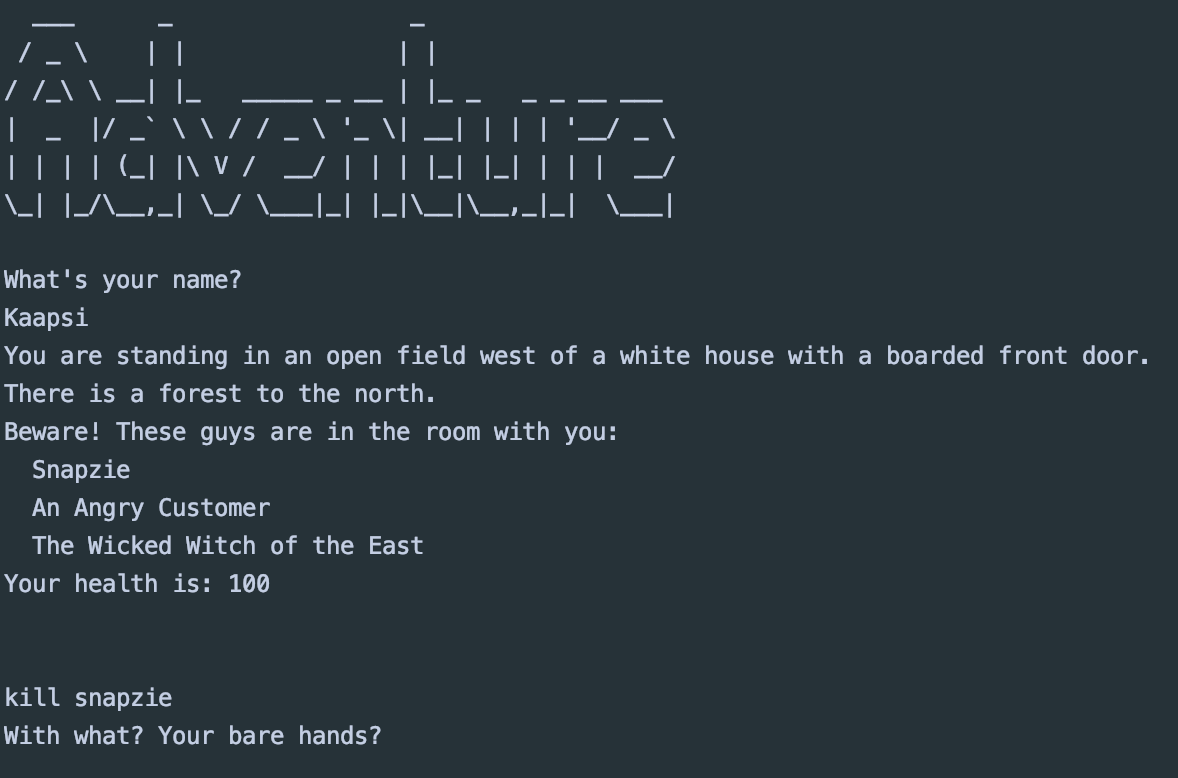
\includegraphics[width=0.9\linewidth]{Materials/Results/PlayersEntering}
	\caption{We see that we cannot attack other players without having the knife.}
	\label{sc2}
\end{figure}

\begin{figure}[H]
	\centering
	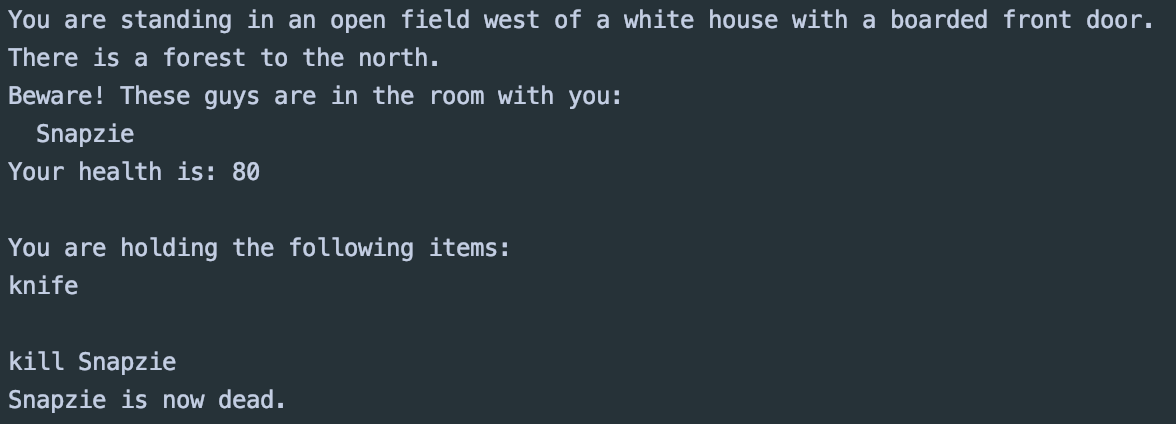
\includegraphics[width=0.8\linewidth]{Materials/Results/AttackingPlayer}
	\caption{We see that the player with the knife can attack other players.}
	\label{sc3}
\end{figure}

But to show off the weather effects and the boss, we have provided to more showcasing images for these variations, namely \autoref{sc4} and \autoref{sc5}.

\begin{figure}[H]
	\centering
	\includegraphics[width=0.6\linewidth]{example-image-a}
	\caption{We see that we cannot attack other players without having the knife.}
	\label{sc4}
\end{figure}

\begin{figure}[H]
	\centering
	\includegraphics[width=0.6\linewidth]{example-image-a}
	\caption{We see that the player with the knife can attack other players.}
	\label{sc5}
\end{figure}